\documentclass[11pt]{article}
\usepackage[margin=1in]{geometry}
\usepackage{graphicx}
\usepackage{booktabs}
\usepackage{hyperref}

\title{Progress Report 2\\Detecting and Mitigating Simple IoT-Based DoS Attacks}
\author{Group 8}
\date{\today}

\begin{document}
\maketitle

\section*{Overview}
This progress report presents the second stage of our IoT-based denial-of-service detection project.
The main focus of this milestone was to strengthen the existing rule-based system so that the
reported results are better aligned with the project scope and more defensible experimentally.
Rather than adding machine learning, this phase improves the reliability of the current pipeline
through corrected time-window alignment, repeatable multi-seed evaluation, detector comparison,
feature ablation, and report-ready visualization.

\section*{Work Completed Since Progress Report 1}
\begin{itemize}
  \item Fixed feature-label alignment so that every labeled second appears in the feature table, including zero-traffic windows.
  \item Updated the feature extraction timeline to align to synthetic traffic seconds rather than the first packet timestamp.
  \item Refactored detection into explicit detector modes: adaptive thresholds and fixed thresholds.
  \item Added a protocol-oriented rule set that separately captures UDP-flood behavior and SYN-flood behavior.
  \item Implemented a multi-seed experiment runner and generated averaged results over 10 seeds.
  \item Added feature ablation experiments to measure the value of different feature subsets.
  \item Added detector-comparison, phase-level, ablation, and multi-seed summary figures.
\end{itemize}

\section*{Methodology Updates}
\textbf{Aligned feature extraction:}
The canonical timeline is now taken from the ground-truth label file. Feature extraction produces
one row per labeled second, and missing traffic windows are filled with zeros. This removes the
row-count mismatch present in the earlier prototype and makes label-feature comparisons exact.

\textbf{Detector comparison:}
Two rule-based detectors are now evaluated:
\begin{itemize}
  \item \textbf{Adaptive thresholds:} rolling baseline mean plus threshold multiplier times standard deviation.
  \item \textbf{Fixed thresholds:} thresholds calibrated from the initial normal-traffic period.
\end{itemize}

\textbf{Decision logic:}
The detector now uses a protocol-oriented rule rather than flagging a window when any single
feature exceeds threshold.
\begin{itemize}
  \item UDP-flood rule: high packets/sec and high bytes/sec.
  \item SYN-flood rule: high SYN/sec and high unique destination ports.
\end{itemize}

\textbf{Evaluation expansion:}
Experiments are now averaged over 10 random seeds. In addition to overall metrics, we also report
phase-specific behavior for normal traffic, benign burst traffic, UDP flood traffic, and SYN flood
traffic. A feature ablation study compares the following sets:
\begin{itemize}
  \item packets only
  \item packets plus bytes
  \item SYN count plus destination-port diversity
  \item full feature set
\end{itemize}

\section*{Current Results}
Table~\ref{tab:detectors} summarizes the averaged detector comparison using the full feature set.
The adaptive detector remains conservative and produces a relatively low false positive rate, but
its recall is still limited. The fixed-threshold detector achieves perfect recall on the simulated
attack phases, but it overreacts to the benign burst phase, which increases the false positive
rate. This tradeoff is important because it highlights the central challenge of the project:
improving attack coverage without treating legitimate spikes as attacks.

\begin{table}[h]
  \centering
  \caption{Averaged detector comparison over 10 seeds}
  \label{tab:detectors}
  \begin{tabular}{lccccc}
    \toprule
    Detector & Accuracy & Precision & Recall & FPR & F1 \\
    \midrule
    Adaptive & 0.7613 & 0.5983 & 0.1375 & 0.0308 & 0.2229 \\
    Fixed & 0.9375 & 0.8000 & 1.0000 & 0.0833 & 0.8889 \\
    \bottomrule
  \end{tabular}
\end{table}

The phase-level results help explain these averages. The adaptive detector keeps false positives
near zero on the normal phases, but it still flags the benign firmware-burst phase in roughly
37\% of windows and detects only a small fraction of the two attack phases. In contrast, the
fixed detector catches both attack phases completely, but it flags the entire benign burst phase.

Table~\ref{tab:ablation} summarizes the averaged ablation results. The full feature set performs
best overall among the adaptive configurations. The packets-only and packets-plus-bytes subsets
produce lower recall, while the SYN-plus-ports subset is very precise but misses most attack
windows because it is only strongly aligned with the SYN-flood behavior.

\begin{table}[h]
  \centering
  \caption{Feature ablation results for the adaptive detector}
  \label{tab:ablation}
  \begin{tabular}{lccccc}
    \toprule
    Feature Set & Accuracy & Precision & Recall & FPR & F1 \\
    \midrule
    Packets only & 0.7488 & 0.4857 & 0.0900 & 0.0317 & 0.1516 \\
    Packets + bytes & 0.7413 & 0.3782 & 0.0575 & 0.0308 & 0.0995 \\
    SYN + ports & 0.7700 & 1.0000 & 0.0800 & 0.0000 & 0.1476 \\
    Full feature set & 0.7612 & 0.5983 & 0.1375 & 0.0308 & 0.2229 \\
    \bottomrule
  \end{tabular}
\end{table}

\section*{Figures}
\begin{figure}[h]
  \centering
  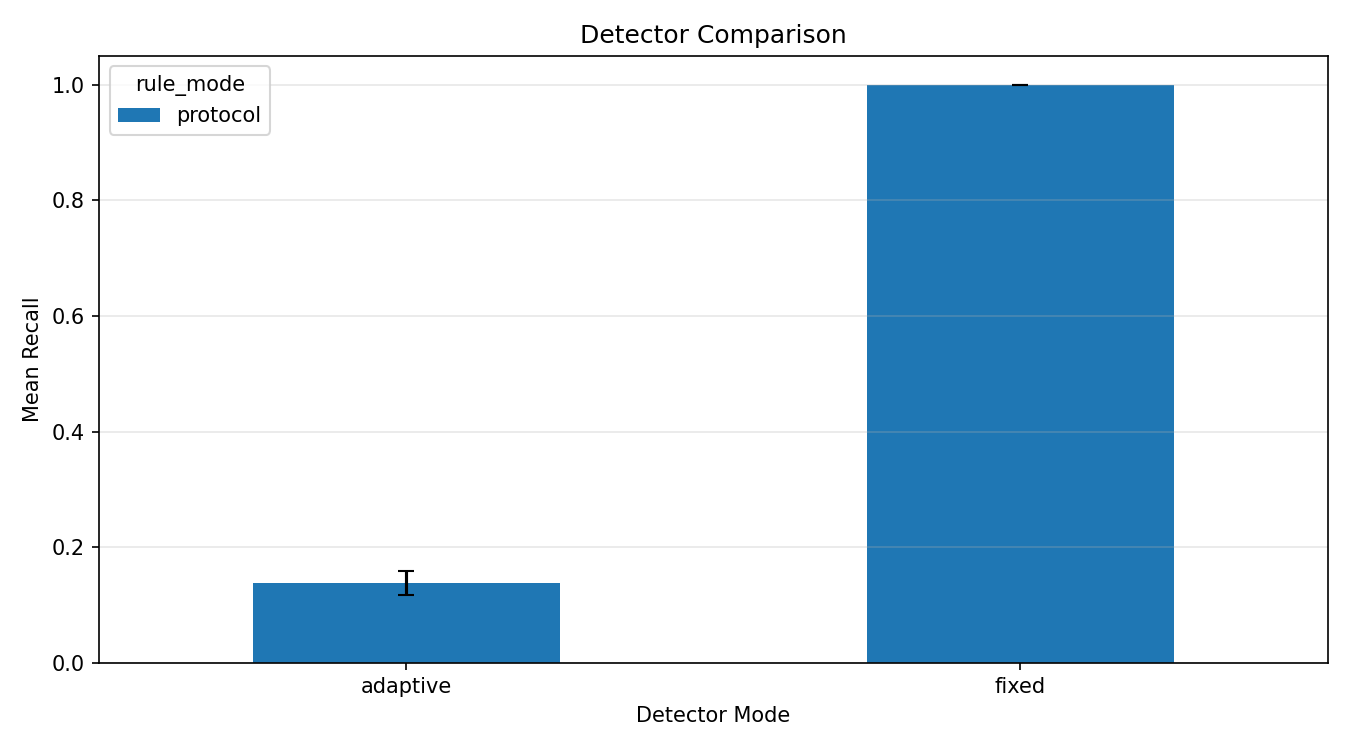
\includegraphics[width=\linewidth]{figures/detector_comparison.png}
  \caption{Detector comparison using averaged multi-seed recall.}
\end{figure}

\begin{figure}[h]
  \centering
  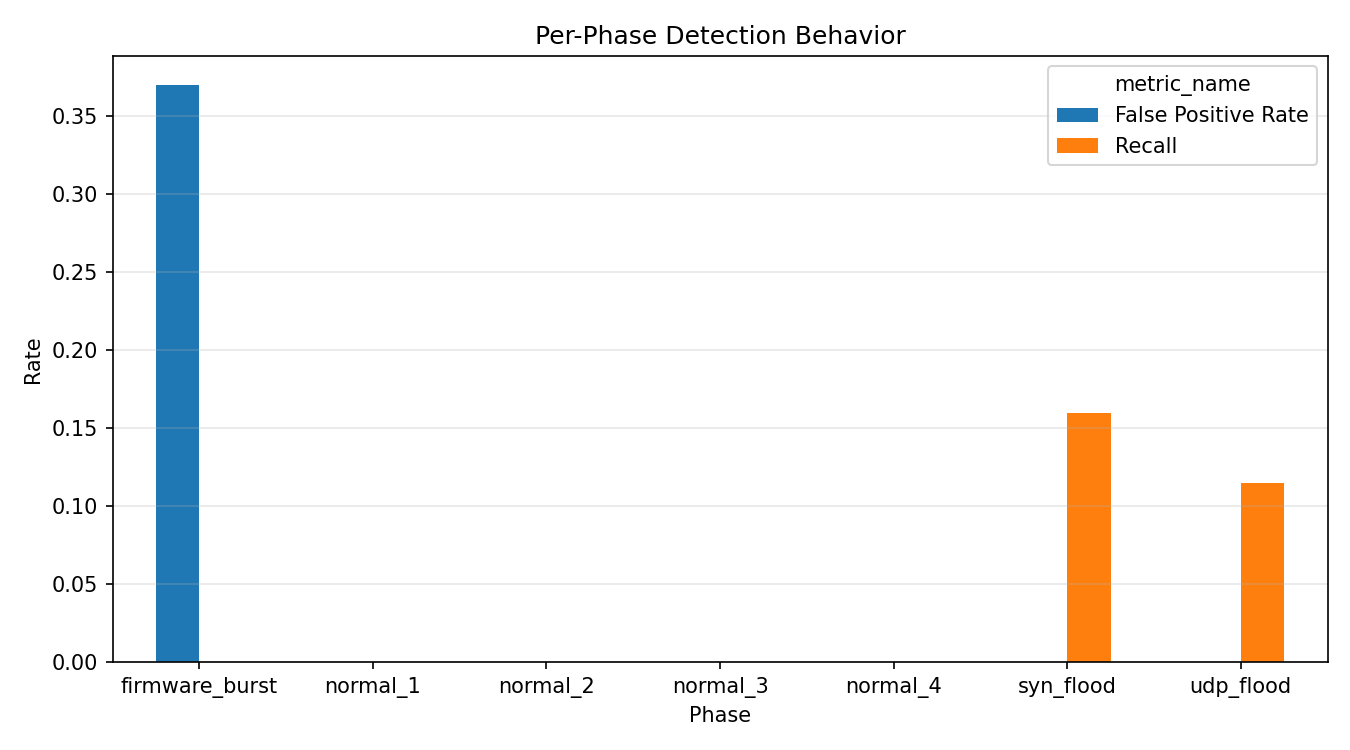
\includegraphics[width=\linewidth]{figures/phase_metrics.png}
  \caption{Per-phase behavior for the primary adaptive detector configuration.}
\end{figure}

\begin{figure}[h]
  \centering
  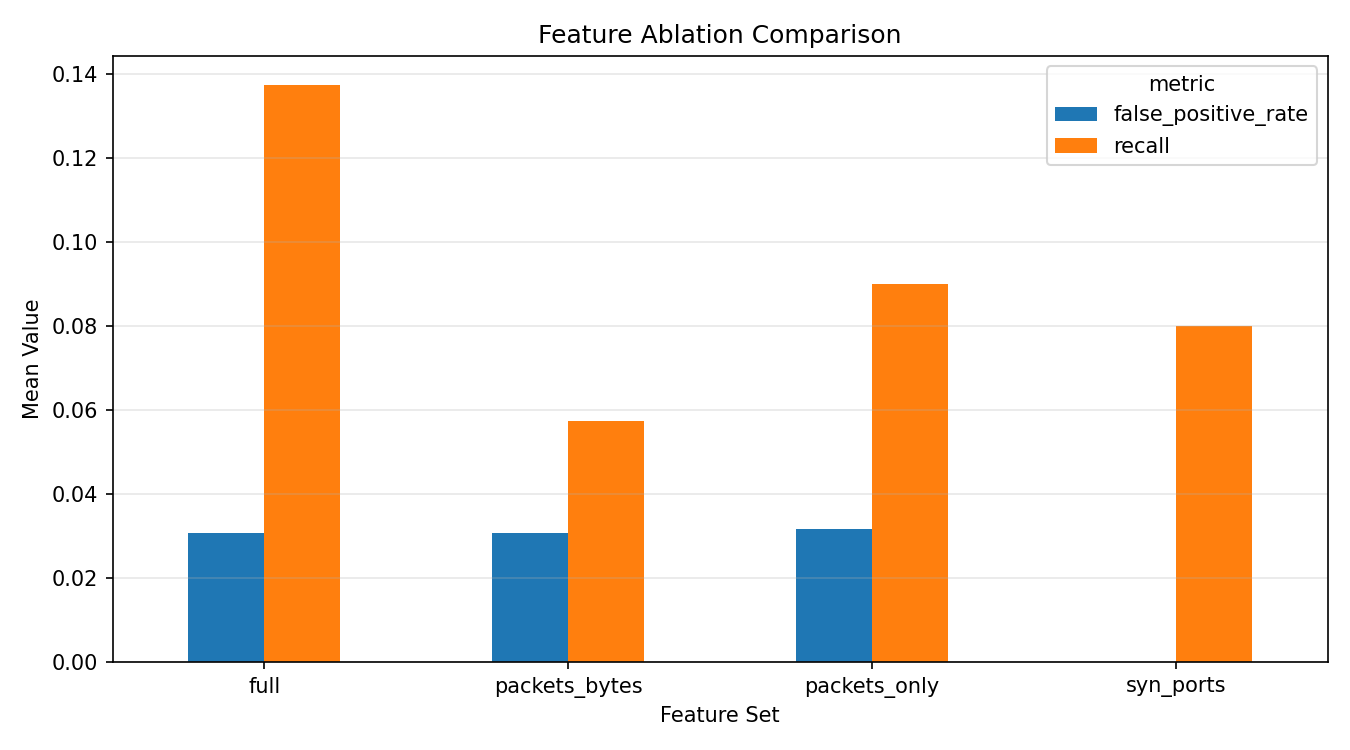
\includegraphics[width=\linewidth]{figures/ablation_comparison.png}
  \caption{Feature ablation comparison for the adaptive detector.}
\end{figure}

\begin{figure}[h]
  \centering
  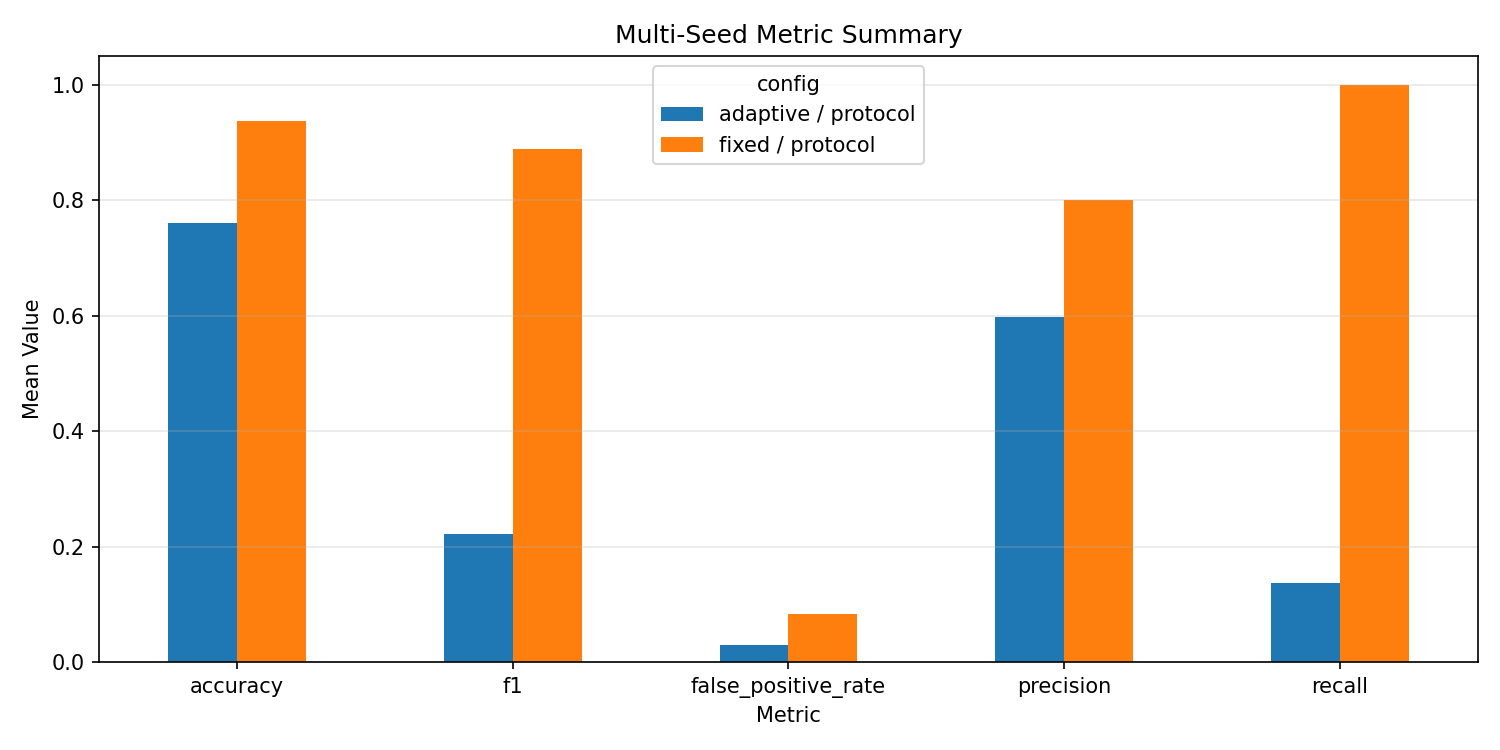
\includegraphics[width=\linewidth]{figures/multi_seed_summary.png}
  \caption{Averaged metrics across detector configurations.}
\end{figure}

\section*{Remaining Issues and Next Steps}
The current results show meaningful progress, but they also reveal the main limitation of the
current design: the project now has a clear tradeoff between detection coverage and false
positives. The adaptive detector is cautious but misses many attack windows, while the fixed
detector is stronger on recall but reacts too aggressively to the benign burst phase.

The remaining work for the final stage of the project will focus on:
\begin{itemize}
  \item tuning thresholds and calibration settings to reduce the benign-burst false positive rate,
  \item testing whether the adaptive detector can be improved without losing interpretability,
  \item refining the final discussion around why different feature groups respond differently to UDP and SYN attacks,
  \item preparing the final report using the new multi-seed results and figures.
\end{itemize}

\section*{Conclusion}
This milestone substantially strengthens the original prototype. The project now includes aligned
feature extraction, fair rule-based detector comparison, multi-seed evaluation, phase-level
analysis, and feature ablation. These improvements make the system more suitable for a course
research report and provide a much stronger basis for the final evaluation and discussion.

\end{document}
